\appendix
\newpage



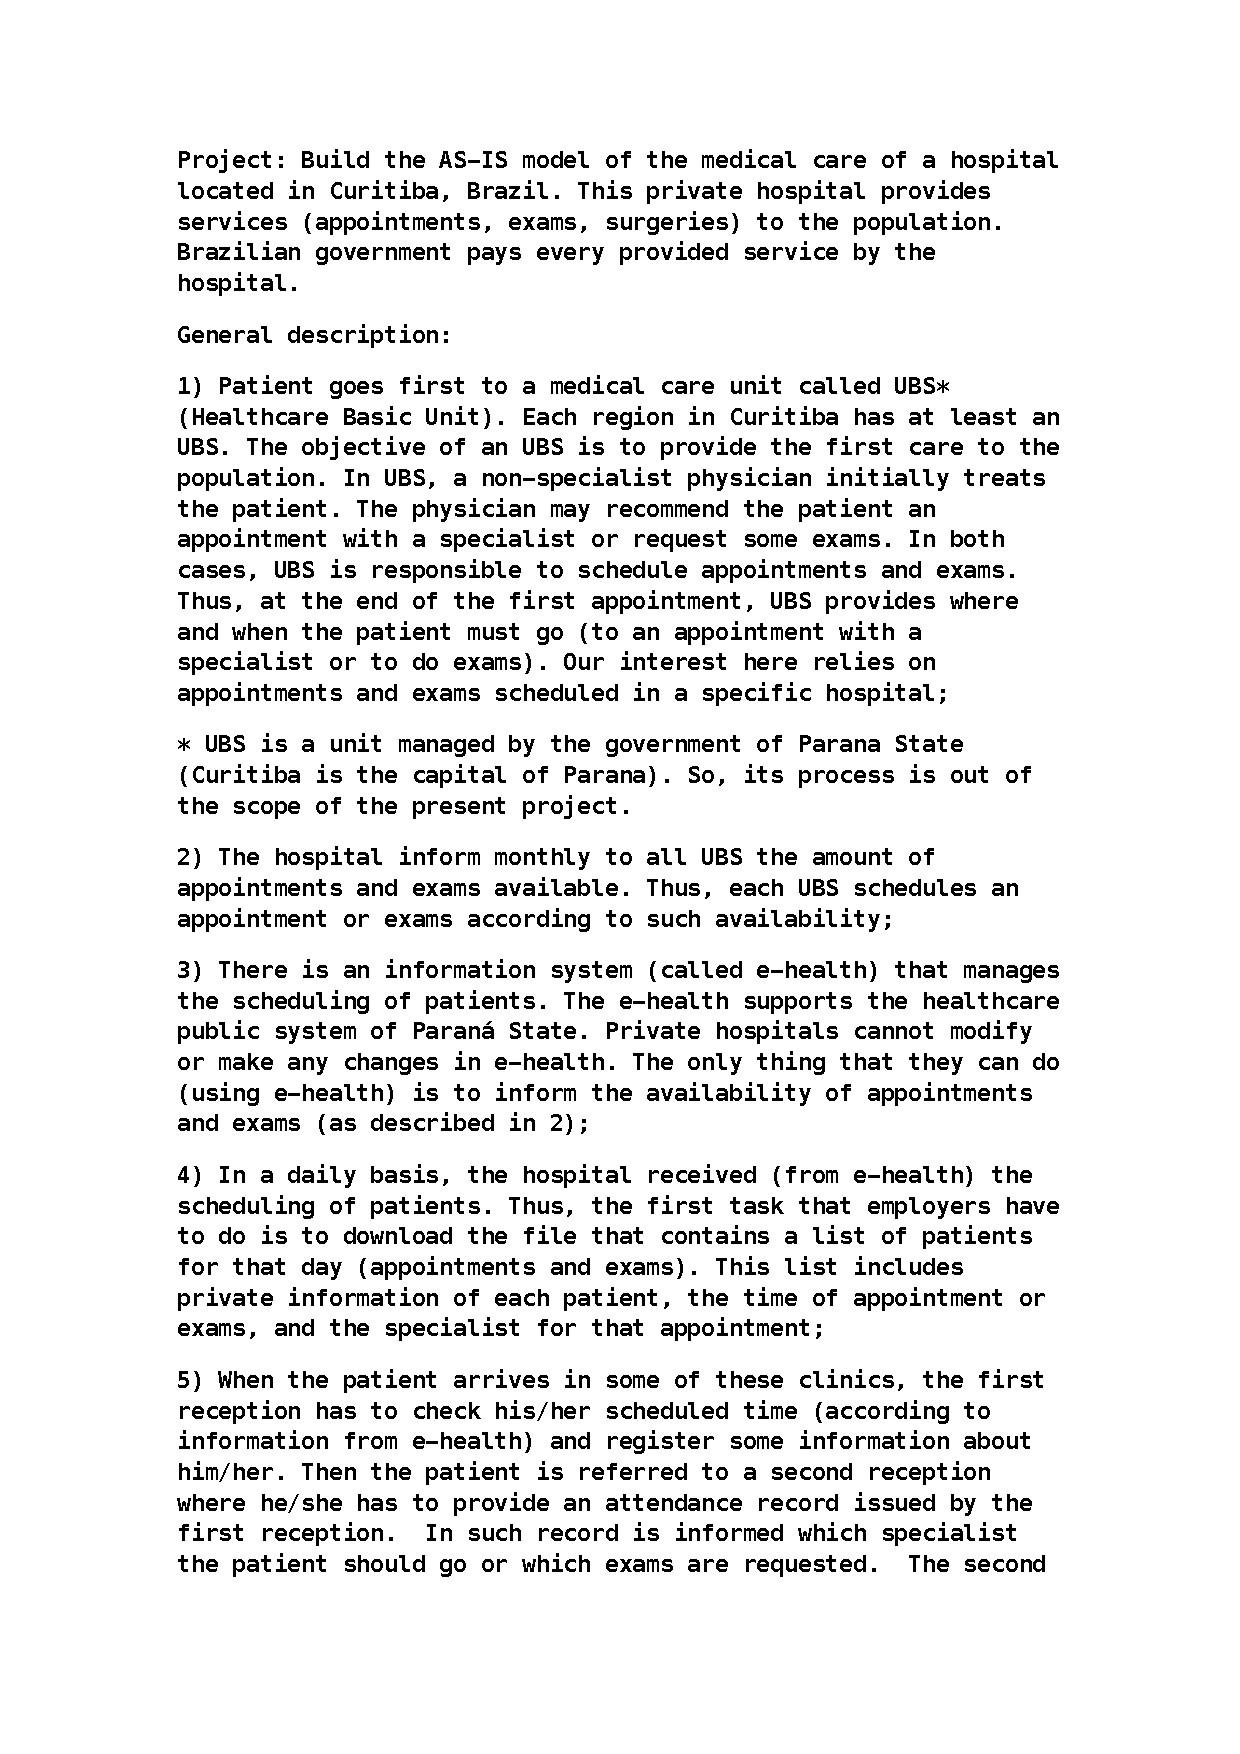
\includepdf[pages=1,scale=0.8,pagecommand=\section{Healthcare Process From Brazil}]{Figures/Appendix/HealthCareProcess.pdf}
\includepdf[pages=2-,scale=0.8]{Figures/Appendix/HealthCareProcess.pdf}

\section{Usermanual for DCR graph parser \label{sec:UsermanualForDcrGraphParser}}
\section{Possible solutions for creating the database \label{sec:SolutionsForCreatingTheDatabaseAppendix}}
The parser has only one window in which a great deal of information can be entered. \\
In the first box, called INPUT FILE, the user can write the path of a DCRGraphs.net XML-file. The user can also browse for such a file using the Choose XML-file button just below it. This will open a defaultWindows Open Dialog. Below the button is a box labeled Workflow Id. This is used by FlowIT to uniquely define a workflow.  \newline
The Workflow Id should not contain spaces or symbols, but numbers, uppercase, and lowercase letters are OK. \newline
The box labeled Workflow Name will be the name of the workflow, which the client presents. Anything can be written in this box, but if the string is too long, the Client will not be able to show everything without scrolling horizontally in the Client user interface. \newline
In the Server Base-URL box needs to know the base URL of the server. \newline
This will be http://flowit.azurewebsites.net/ when publishing workflows onto the hosted Azure FlowIT server. It will be http://localhost:13768/ when posting to the local IIS instance when running FlowIT locally (Remember to change the Client Settings file, when running locally). \newline
The Event Base-URLs will be the base address(es) of the Event-Machines meant to host the workflow. For localhost usage it will be http://localhost:13752/ (the two localhost-ports can be changed through Visual Studio or IIS-settings if desired, these are the ports the projects are configured for).  \newline
For the hosted Azure Event Machines the addresses will be one or more of http://flowites1.azurewebsites.net/ http://flowites2.azurewebsites.net/ http://flowites3.azurewebsites.net/ or http://flowites4.azurewebsites.net/. If multiple Event Machines are desired put a comma between the base-addresses. The input is not checked before usage, so be careful what is typed into these fields. \newline
The last textbox is the password chosen for all of the default users, which are the actors or roles from the DCRGraphs.net XML-file. \newline
Before we get to the buttons there are two checkboxes. These are almost self-explanatory. The first one will try to create the workflow on the chosen server. This will fail if the workflow exists already. \newline
The second one will create the users with the typed in password, if the users does not already exist. In the case where the users are existing, the parser will not change the passwords of the existing users, it will just add the roles to the users. \newline
The leftmost button in the bottom of the window, will parse the selected XML-file and turn it into JSON-objects which are then saved as text in graph.json which will be written to disk in the same folder as the parser-executable. \newline
The other button will upload the parsed data directly into the Flow IT system, based on the parameters given.
